\documentclass[a4paper]{article}
\usepackage{graphicx}
\usepackage[margin = 1in]{geometry}
\usepackage{ragged2e}
\usepackage[hidelinks, colorlinks = true, citecolor = black, linkcolor = blue]{hyperref}
\usepackage{parskip}
\usepackage{cite}
\usepackage{cellspace}
\usepackage{makecell}
\usepackage{mwe}
\setlength\cellspacetoplimit{4pt}
\setlength\cellspacebottomlimit{4pt}
\usepackage{caption} 
\usepackage{pgfplots}
\usepackage{amsmath}
\usepackage{tikz}
\usepackage{pdfpages}
\newcommand{\inv}{^{\raisebox{.2ex}{$\scriptscriptstyle-1$}}}
\newcommand{\unit}[1]{~\mathrm{#1}}
\captionsetup[table]{skip=10pt}
\renewcommand{\arraystretch}{1.5}


\usepackage{tikz}
\usetikzlibrary{shapes,arrows,positioning,fit,backgrounds,calc}
\usepackage{pgfplots}
\pgfplotsset{compat=1.16}
\pgfplotsset{ignore zero/.style={%
  #1ticklabel={\ifdim\tick pt=0pt \else\pgfmathprintnumber{\tick}\fi}
}}
\usepackage{pgf}
\begin{document}
\section{Introduction}
A potentiometer is an electrical component that can be used both as a variable
resistor, and as a voltage divider. The aim of the experiments described in this
report is to analyze the behaviour of the potentiometer.
\section{Background/Theory}
A potentiometer is a resistor that has three terminals. Two of the terminals
constitute the full resistance value, while the third one is a sliding contact.
Figure 1 displays the different contacts of the potentiometer.
\begin{figure}[!ht]
    \begin{minipage}{0.4\textwidth}
        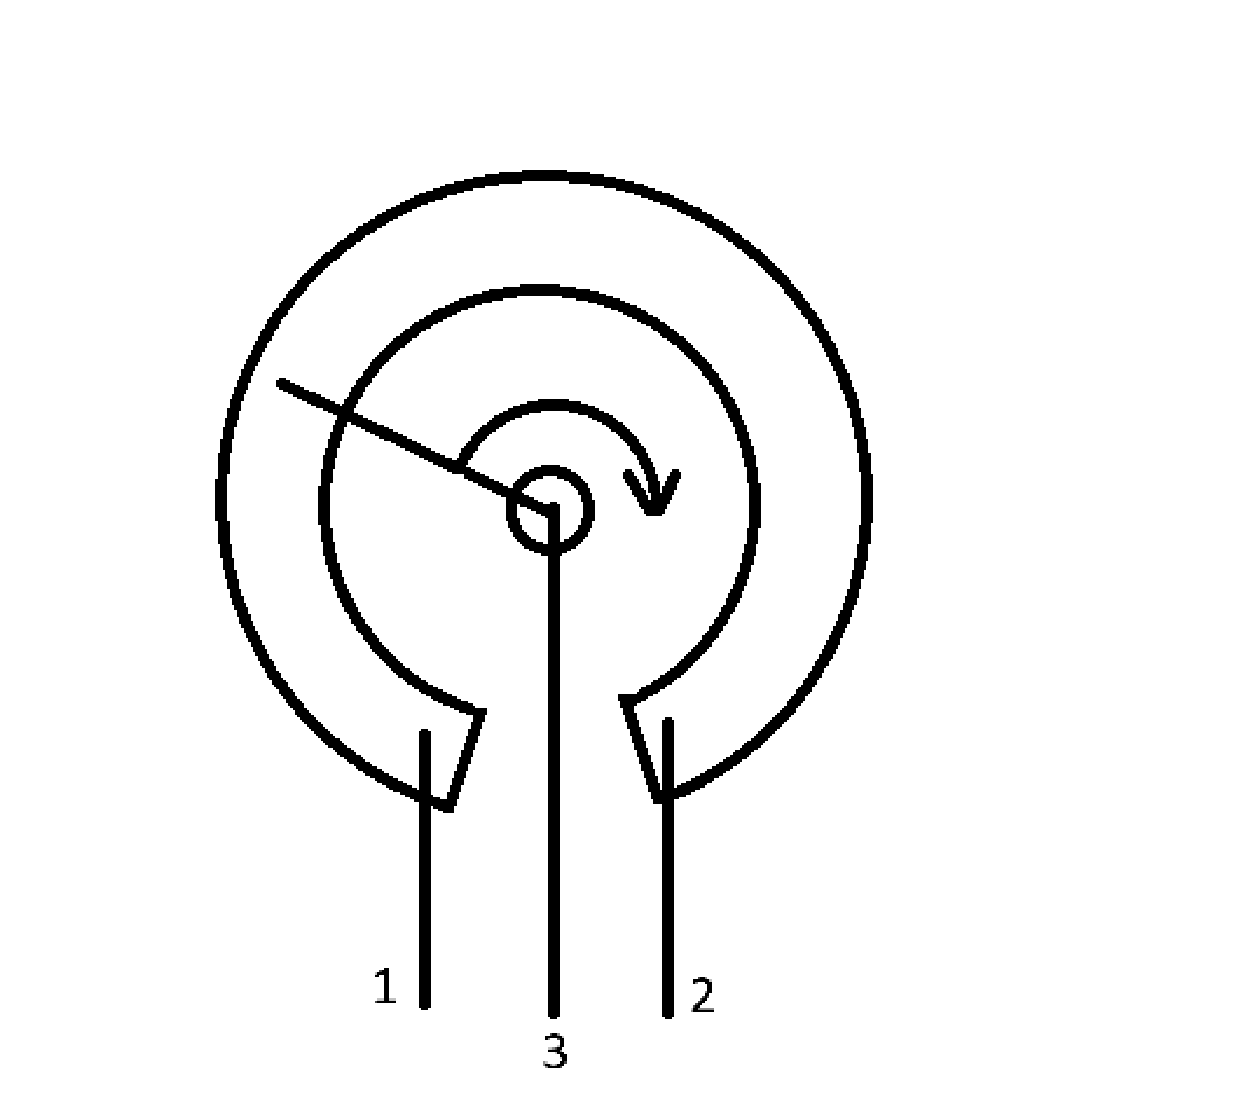
\includegraphics[width = \textwidth]{potterminals.png}
       \label{fig:1}
        \caption{Drawing of a potentiometer with labeled terminals}    
    \end{minipage}
\end{figure}

The resistance between terminals 1 and 2 is constant, while the resistance
between 1 and 3 is determined by the following equation:
\begin{equation}
    R_{13} = kR
\end{equation}
%ref

Since the potentiometer can be used as a voltage divider, the value of the
potential difference between terminals 1 and 3 will be determined by:
\begin{equation}
    V_{13} = k V_{tot}
\end{equation} 

When adding a load resistor in parallel to terminals 1 and 3, the voltage across
them becomes:
\begin{equation}
    V_{13} = \frac{kR_{13}}{R_{13}+k(1-k)R_p} V
\end{equation}
\section{Methods \& Materials}

\subsection{Experimental Set-Up unloaded potentiometer}

\subsection{Experimental Set-Up with fixed resistor}

\subsection{Experimental Set-Up with fixed load current}
\section{The Unloaded Potentiometer}
\subsection{Measurement Results}
Table 1 displays the measured voltage values in terms of k, also displaying the
theoretical voltage.
\begin{table}[!ht]
    \centering
    \label{tab:1}
    \caption{Measured and expected voltage in terms of K}
    \begin{tabular}{|c|c|c|c|} 
    \hline
    $k$ & \makecell{$Measured~V$ \\ V} & \makecell{$\Delta V$ \\ V} &
    \makecell{$Expected~V$ \\ V}  \\ 
    \hline
    0.1                                       & 0.302      &  0.009          & 0.296      \\
    0.2                                       & 0.594      &   0.009         & 0.592      \\
    0.3                                       & 0.89       &   0.017         & 0.888      \\
    0.4                                       & 1.184      &  0.014          & 1.184      \\
    0.5                                       & 1.481      &  0.013          & 1.480     \\
    0.6                                       & 1.776      &  0.021          & 1.775      \\
    0.7                                       & 2.076      &  0.023          & 2.071      \\
    0.8                                       & 2.365      &  0.024          & 2.367      \\
    0.9                                       & 2.663      &  0.025          & 2.663      \\
    1                                         & 2.957      &  0.031          & 2.959       \\
    \hline
    \end{tabular}
    \end{table}
\subsection{Graphs}
Figure 4 displays the measured voltage in terms of K.
\begin{figure}[!ht]
    \centering
    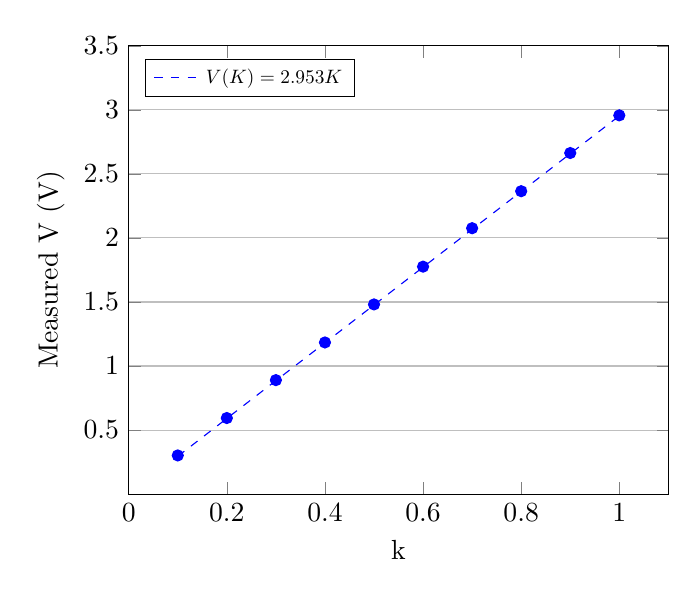
\begin{tikzpicture}
        \begin{axis}[legend pos = north west, legend style={nodes={scale=0.7}}, ymajorgrids = true, domain = 0.1:1, xmin = 0, xlabel = k, xtick = {0, 0.2, 0.4, 0.6, 0.8, 1.0, 1.2}, ymin = 0, ymax = 3.5, ytick = {0, 0.5, 1, 1.5, 2, 2.5, 3, 3.5}, ylabel = Measured V$ \unit{(V)}$, ignore zero = y]
        
        \addplot[blue, samples = 100, dashed]{2.953*x};
        \addplot  [only marks, color = blue] coordinates {
            (0.1, 0.302)
            (0.2, 0.594)
            (0.3, 0.89)
            (0.4, 1.184)
            (0.5, 1.481)
            (0.6, 1.776)
            (0.7, 2.076)
            (0.8, 2.365)
            (0.9, 2.663)
            (1, 2.957)
            
        };
        
        \legend{$V(K) = 2.953K$ }
        \end{axis}
    \end{tikzpicture}
    \caption{Velocity of the slat in terms of time}
    \label{fig:3}
\end{figure}
\subsection{Discussion}
The main goal of this experiment was to determine the effect of changing the
k-value of the potentiometer on the voltage load of the varying resistance. When
looking at the graphical representation of these values seen on figure 3, we see
a linear relationship between the k-value and the voltage drop on the
potentiometer. Analyzing the difference between the measured and expected
voltage, we see that the measured values are accurate, as the difference between
them and the expected values falls within the measurement error. 
\newpage
\section{Potentiometer loaded with fixed resistor}
\subsection{Measurement results}
Table 2 displays the measurements for K,
the unloaded potentiometer value, both loads, with their measured and
theoretical values, and percent deviations.
\begin{table}[!ht]
    \centering
    \label{tab:2}
    \caption{Measured and theoretical load values in terms of K}
    \begin{tabular}{|c|c|c|c|c|c|c|c|} 
    \hline
    $k$ & \makecell{$Unloaded~ V$\\ V} & \makecell{$Load~1$\\ V} & \makecell{$Load~1~
      theoretical$\\ V} & \makecell{$PD~1$\\ \%}  & \makecell{$Load~2$\\ V} &
      \makecell{$Load~2~theoretical$\\ V}
       & \makecell{$PD~2$ \\ \%}   \\ 
    \hline
    0.1     & 3        & 0.274  & 0.156                & 75.85 & 0.253  & 0.111                & 56.02  \\
    0.2     & 3        & 0.514  & 0.329                & 56.27 & 0.451  & 0.239                & 46.98  \\
    0.3     & 3        & 0.739  & 0.522                & 41.46 & 0.628  & 0.388                & 38.28  \\
    0.4     & 3        & 0.957  & 0.740                & 29.32 & 0.809  & 0.562                & 30.53  \\
    0.5     & 3        & 1.184  & 0.987                & 20.00 & 0.993  & 0.770                & 22.47  \\
    0.6     & 3        & 1.433  & 1.269                & 12.97 & 1.21   & 1.022                & 15.55  \\
    0.7     & 3        & 1.717  & 1.594                & 7.74  & 1.47   & 1.334                & 9.27   \\
    0.8     & 3        & 2.039  & 1.973                & 3.35  & 1.801  & 1.730                & 3.97   \\
    0.9     & 3        & 2.448  & 2.421                & 1.11  & 2.268  & 2.249                & 0.86   \\
    1       & 3        & 2.952  & 2.959                & 0.24  & 2.948  & 2.959                & 0.37   \\
    \hline
    \end{tabular}
    \end{table}
\subsection{Graphs}
Figure 5 displays the voltage across the load resistor in terms of K, comparing
them to the theoretical values, and the
voltage drop on the unloaded potentiometer.
\begin{figure}[!ht]
    \centering
    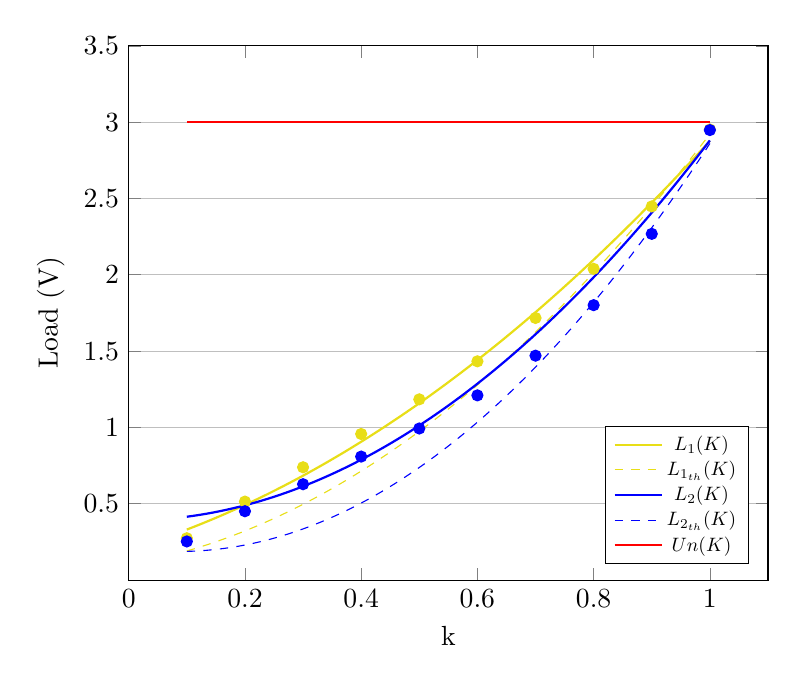
\begin{tikzpicture}
        \begin{axis}[width = 0.8\textwidth, legend pos = south east, legend style={nodes={scale=0.7}}, ymajorgrids = true, domain = 0.1:1, xmin = 0, xlabel = k, xtick = {0, 0.2, 0.4, 0.6, 0.8, 1.0, 1.2}, ymin = 0, ymax = 3.5, ytick = {0, 0.5, 1, 1.5, 2, 2.5, 3, 3.5}, ylabel = Load$ \unit{(V)}$, ignore zero = y, ]
        
        \addplot[black!10!yellow, thick, samples = 100]{1.52*(x^2) + 1.157*x +0.2};
        \addplot  [only marks, color = black!10!yellow, forget plot] coordinates {
            (0.1,	0.274)
            (0.2,	0.514)
            (0.3,	0.739)
            (0.4,	0.957)
            (0.5,	1.184)
            (0.6,	1.433)
            (0.7,	1.717)
            (0.8,	2.039)
            (0.9,	2.448)
            (1,	2.952)

            
        };
         
        \addplot[black!10!yellow, thin, samples = 100, dashed]{2.15*(x^2) + 0.67 * x +
        0.102};
        \addplot[blue, thick, samples=100]{2.49*(x^2) + 0.39};
        \addplot  [only marks, color = blue, forget plot] coordinates {
            (0.1,	0.253)
            (0.2,	0.451)
            (0.3,	0.628)
            (0.4,	0.809)
            (0.5,	0.993)
            (0.6,	1.21)
            (0.7,	1.47)
            (0.8,	1.801)
            (0.9,	2.268)
            (1,	2.948)
            

            
        };
        \addplot[blue, thin, samples=100, dashed]{3.19*(x^2) - 0.54 * x + 0.21};
        \addplot[red, thick, samples = 100]{3};
        \legend{$L_1(K)$, $L_{1_{th}}(K)$,$L_2(K)$,$L_{2_{th}}(K)$,$Un(K)$}
        \end{axis}
    \end{tikzpicture}
    \label{fig:5}
    \caption{Loads in terms of k}
\end{figure}
\par 
Figure 6 displays the relationship between percent deviation and K.
\begin{figure}
    \centering
    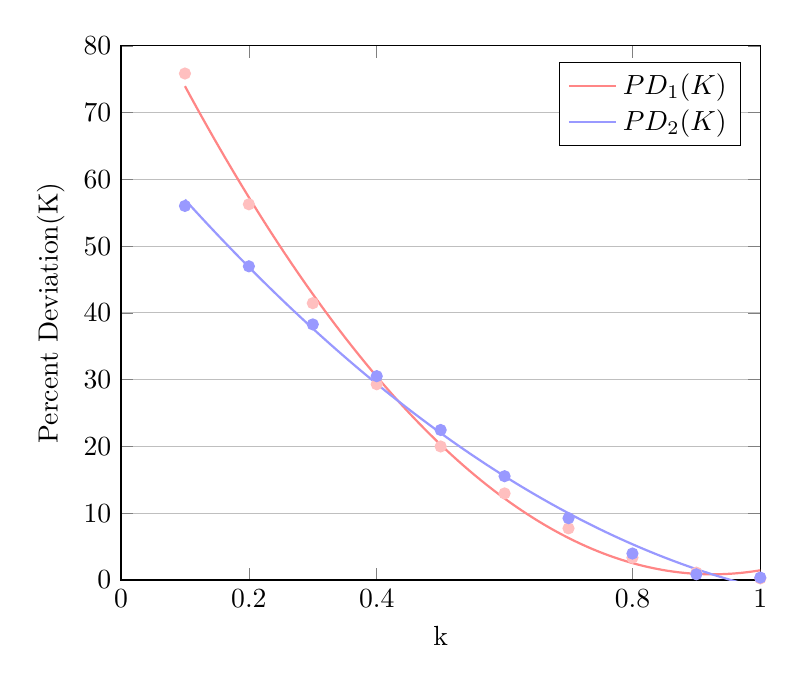
\begin{tikzpicture}
        \begin{axis}[width = 0.8\textwidth, legend pos = north east, legend style={nodes={scale=1}},
        ymajorgrids = true, domain = 0.1:1, xmin = 0, xmax = 1, ymin = 0, ymax =
        80, xlabel = k, xtick = {0, 0.2, 0.4, 0.8, 1}, ytick = {0, 10, 20, 30,
        40, 50, 60, 70, 80}, ylabel = Percent Deviation(K)]
        \addplot[red!30!pink, thick, samples = 100]{107.36*(x^2) - 198.65*x +92.75};
        \addplot[only marks, color = pink, forget plot] 
        coordinates {
            (0.1,	75.85)
            (0.2,	56.27)
            (0.3,	41.46)
            (0.4,	29.32)
            (0.5,	20.00)
            (0.6,	12.97)
            (0.7,	7.74)
            (0.8,	3.35)
            (0.9,	1.11)
            (1,	0.24)
             
        };
        \addplot[white!60!blue, thick, samples = 100]{45.56*(x^2) - 114.72*x + 67.98};
        \addplot[only marks, color = white!60!blue, forget plot] 
        coordinates{    
        (0.1,	56.02)
        (0.2,	46.98)
        (0.3,	38.28)
        (0.4,	30.53)
        (0.5,	22.47)
        (0.6,	15.55)
        (0.7,	9.27)
        (0.8,	3.97)
        (0.9,	0.86)
        (1,	0.37)
        };
        \legend{$PD_ 1(K)$,$PD_2(K)$}
        \end{axis}
    \end{tikzpicture}
    \label{fig:6}
    \caption{Percent deviation in terms of k}
\end{figure}
\subsection{Discussion}
\end{document}